\documentclass[journal]{IEEEtran}
\usepackage{amsmath,amsfonts,amssymb,amsthm,bm}
\usepackage{booktabs,tabularx}
\usepackage{graphicx}
\usepackage{tikz}
\pgfdeclarelayer{background}
\pgfsetlayers{background,main}
\usetikzlibrary{shapes.geometric,arrows.meta,positioning}
\usepackage{hyperref}

\newtheorem{theorem}{Theorem}
\newtheorem{definition}{Definition}
\newtheorem{remark}{Remark}

\title{Scale-Invariant Contraction Hierarchies: Group-Theoretic Cohesion, Coupling Augmentation, and Compactness Propagation}
\author{Richard~Sherman,~\IEEEmembership{Member,~IEEE}%
\thanks{R. Sherman is with the System Architecture Invariant Manifest Group, Keller, TX 76248 USA.}}

\begin{document}
\maketitle

\begin{abstract}
Multi-area inverter-dominated power grids and autonomous multi-agent swarms exhibit structural self-similarity across fast device, intermediate cluster, and slow supervisory timescales. This paper formalizes a scale-invariant control theory built on four pillars: (1) finite symmetry group equivariance characterizing allowable cohesive configurations ($\mathbf{C}_\ell$) versus symmetry-breaking external coupling interfaces ($\mathbf{P}_\ell$), together with state augmentation converting coupling into internal cohesion; (2) a Renormalization Group (RG) formulation of top-level reserve margin ($\Delta P_{\text{crit}} > 0$) balancing economic cost minimization ($J_{\text{cost}}$) against disruption minimization ($J_{\text{disrupt}}$); (3) time-reversible adjoint flows and stroboscopic singular perturbation lifting continuous dynamics to Nekrashevych self-similar discrete-event trees; and (4) inductive preservation of closedness and compactness across all contracting layers, contrasted with fractal reachable boundaries in the unstable odometer regime.
\end{abstract}

\section{Explicit Trajectory Dynamics: Cohesion vs. Coupling}
Consider an $L$-layer hierarchical network evolving over continuous time $t \in \mathbb{R}_{\ge 0}$. At layer $\ell \in \{1, \dots, L\}$, the network comprises $N_\ell$ interconnected nonlinear subsystems. For every subsystem $i \in \{1, \dots, N_\ell\}$, the local state $x_{\ell,i}(t) \in \mathbb{R}^{n_\ell}$ obeys:
\begin{equation}
\dot{x}_{\ell,i}(t) = f_{\ell,i}\big(x_{\ell,i}(t), x_{\ell,\mathcal{N}_i}(t), \hat{\theta}_{\ell,i}(t)\big) + B_{\ell,i} u_{\ell,i}(t) + E_{\ell,i} v_{\ell,i}(t) + \Delta_{\ell,i} w_{\ell,i}(t)
\end{equation}
where $u_{\ell,i}(t)$ is the local control input, $v_{\ell,i}(t)$ is an exogenous interface input from external modules, and $w_{\ell,i}(t)$ is an $L_2$-bounded disturbance. Stacking all $N_\ell$ subsystems yields the full layer-$\ell$ state vector $x_\ell(t) = (x_{\ell,1}(t), \dots, x_{\ell,N_\ell}(t)) \in \mathcal{X}_\ell \subset \mathbb{R}^{N_\ell n_\ell}$, where a trajectory at layer $\ell$ is an absolutely continuous map $x_\ell : [0, \infty) \to \mathcal{X}_\ell$.

\begin{definition}[Cohesion Symmetry Group and Allowable Configurations]
Let $\mathcal{G}_\ell \le S_{N_\ell}$ be the subgroup of subsystem permutations $P_g$ that preserve the layer-$\ell$ internal interaction matrix $\mathbf{C}_\ell$, i.e., $P_g \mathbf{C}_\ell P_g^\top = \mathbf{C}_\ell$ for all $g \in \mathcal{G}_\ell$. When $v_\ell \equiv 0$, the layer-$\ell$ dynamics are $\mathcal{G}_\ell$-cohesive if permuting states, inputs, and parameters commutes with the vector field:
\begin{equation}
f_\ell(P_g x_\ell, P_g u_\ell, P_g \hat{\theta}_\ell) = P_g f_\ell(x_\ell, u_\ell, \hat{\theta}_\ell), \qquad \forall g \in \mathcal{G}_\ell.
\end{equation}
Thus, $\mathbf{C}_\ell$ and $\mathcal{G}_\ell$ define the set of \emph{allowable configurations} preserving internal network coherence.
\end{definition}

\begin{definition}[External Interface Coupling]
An interaction is termed \emph{coupling} ($\mathbf{P}_\ell$) when subsystem $i$ receives an exogenous signal $v_{\ell,i}(t) = h_{\ell,i}(y_{\text{ext}}(t))$ generated by an external module or synchronization channel (such as a Phase-Locked Loop or range-sensor lag) whose dynamics lie outside $\mathcal{X}_\ell$, thereby breaking $\mathcal{G}_\ell$-equivariance:
\begin{equation}
P_g E_\ell v_\ell(t) \neq E_\ell v_\ell(t) \quad \text{for at least one } g \in \mathcal{G}_\ell.
\end{equation}
\end{definition}

\begin{figure*}[!t]
\centering
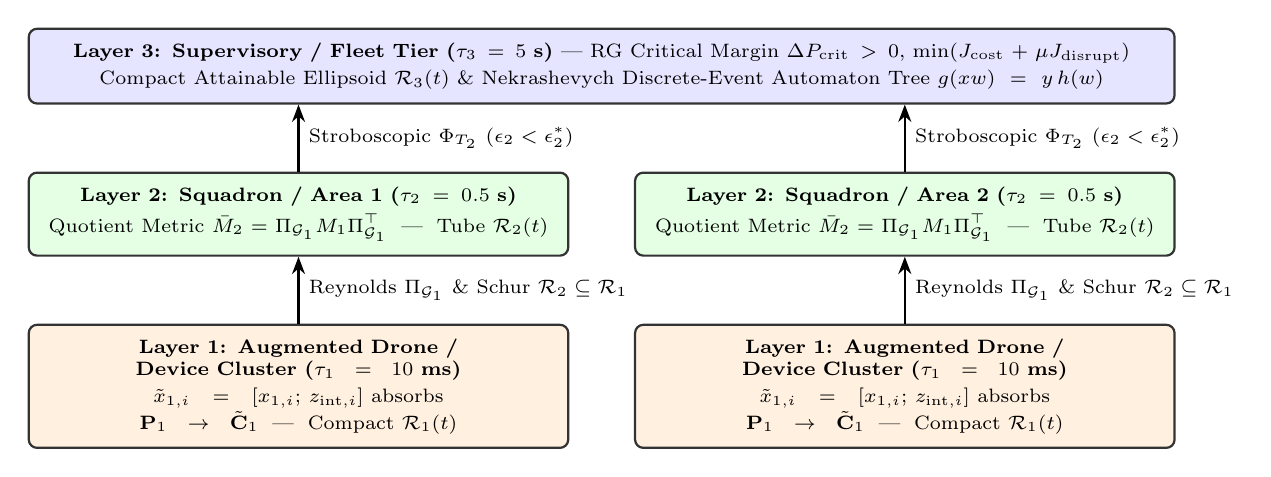
\begin{tikzpicture}[
    node distance=0.85cm and 0.9cm,
    box/.style={rectangle, draw=black!80, thick, rounded corners=3pt, align=center, inner sep=5pt, font=\scriptsize},
    l3/.style={box, fill=blue!10, text width=14.2cm},
    l2/.style={box, fill=green!10, text width=6.5cm},
    l1/.style={box, fill=orange!12, text width=6.5cm},
    arr/.style={-{Stealth[length=2.2mm]}, thick}
]
\node[l3] (fleet) {\textbf{Layer 3: Supervisory / Fleet Tier ($\tau_3 = 5\text{ s}$)} --- RG Critical Margin $\Delta P_{\text{crit}} > 0$, $\min (J_{\text{cost}} + \mu J_{\text{disrupt}})$\\[2pt]Compact Attainable Ellipsoid $\mathcal{R}_3(t)$ \& Nekrashevych Discrete-Event Automaton Tree $g(xw) = y\,h(w)$};

\node[l2, below=0.85cm of fleet.south west, anchor=north west] (sq1) {\textbf{Layer 2: Squadron / Area 1 ($\tau_2 = 0.5\text{ s}$)}\\[2pt]Quotient Metric $\bar{M}_2 = \Pi_{\mathcal{G}_1} M_1 \Pi_{\mathcal{G}_1}^\top$ \;|\; Tube $\mathcal{R}_2(t)$};
\node[l2, below=0.85cm of fleet.south east, anchor=north east] (sq2) {\textbf{Layer 2: Squadron / Area 2 ($\tau_2 = 0.5\text{ s}$)}\\[2pt]Quotient Metric $\bar{M}_2 = \Pi_{\mathcal{G}_1} M_1 \Pi_{\mathcal{G}_1}^\top$ \;|\; Tube $\mathcal{R}_2(t)$};

\node[l1, below=0.85cm of sq1] (dr1) {\textbf{Layer 1: Augmented Drone / Device Cluster ($\tau_1 = 10\text{ ms}$)}\\[2pt]$\tilde{x}_{1,i} = [x_{1,i};\, z_{\text{int},i}]$ absorbs $\mathbf{P}_1 \to \tilde{\mathbf{C}}_1$ \;|\; Compact $\mathcal{R}_1(t)$};
\node[l1, below=0.85cm of sq2] (dr2) {\textbf{Layer 1: Augmented Drone / Device Cluster ($\tau_1 = 10\text{ ms}$)}\\[2pt]$\tilde{x}_{1,i} = [x_{1,i};\, z_{\text{int},i}]$ absorbs $\mathbf{P}_1 \to \tilde{\mathbf{C}}_1$ \;|\; Compact $\mathcal{R}_1(t)$};

\draw[arr] (dr1.north) -- node[right, font=\scriptsize] {Reynolds $\Pi_{\mathcal{G}_1}$ \& Schur $\mathcal{R}_2 \subseteq \mathcal{R}_1$} (sq1.south);
\draw[arr] (dr2.north) -- node[right, font=\scriptsize] {Reynolds $\Pi_{\mathcal{G}_1}$ \& Schur $\mathcal{R}_2 \subseteq \mathcal{R}_1$} (sq2.south);
\draw[arr] (sq1.north) -- node[right, font=\scriptsize] {Stroboscopic $\Phi_{T_2}$ ($\epsilon_2 < \epsilon_2^*$)} (fleet.south -| sq1.north);
\draw[arr] (sq2.north) -- node[right, font=\scriptsize] {Stroboscopic $\Phi_{T_2}$ ($\epsilon_2 < \epsilon_2^*$)} (fleet.south -| sq2.north);
\end{tikzpicture}
\caption{Scale-invariant three-tier contraction hierarchy illustrated on a 3-tier Autonomous Drone Swarm (\texttt{Drone -> Squadron -> Fleet}) and isomorphic multi-area grid. State augmentation converts external coupling $\mathbf{P}_1$ into internal cohesion $\tilde{\mathbf{C}}_1$, while Reynolds projection, stroboscopic lifting, and Schur-complement inclusion propagate compactness upward.}
\label{fig:scale_invariant_arch}
\end{figure*}

We distinguish the static algebraic \emph{cohesive configuration subspace} $\mathcal{X}_\ell^{\mathcal{G}_\ell} \triangleq \{x_\ell \in \mathcal{X}_\ell \mid P_g x_\ell = x_\ell \;\forall g \in \mathcal{G}_\ell\}$ from dynamic \emph{temporal synchronization}, which holds when $\lim_{t \to \infty} d_{M_\ell}(x_\ell(t), \mathcal{X}_\ell^{\mathcal{G}_\ell}) = 0$. Let $\Pi_{\mathcal{G}_\ell} x_\ell = \frac{1}{|\mathcal{G}_\ell|} \sum_{g \in \mathcal{G}_\ell} P_g x_\ell$ denote the Reynolds projector onto $\mathcal{X}_\ell^{\mathcal{G}_\ell}$.

\begin{theorem}[Quotient Contraction Isomorphism]
If layer $\ell$ admits a $\mathcal{G}_\ell$-invariant separable Riemannian metric $M_\ell(x_\ell, \hat{\theta}_\ell)$ ($P_g M_\ell P_g^\top = M_\ell$) with exponential contraction rate $\lambda_\ell > 0$, then: (1) $\mathcal{X}_\ell^{\mathcal{G}_\ell}$ is forward invariant and all trajectories $x_\ell(t)$ synchronize exponentially to $\mathcal{X}_\ell^{\mathcal{G}_\ell}$ as $t \to \infty$; and (2) the renormalized quotient metric $\bar{M}_{\ell+1} = \Pi_{\mathcal{G}_\ell} M_\ell \Pi_{\mathcal{G}_\ell}^\top$ preserves the exact separable Linear Matrix Inequality (LMI) structure at layer $\ell+1$.
\end{theorem}

\section{Renormalization Group Objectives and Coupling Augmentation}
In statistical physics, a Renormalization Group (RG) transformation $V'(\Phi) = \mathcal{R}V(\Phi)$ coarse-grains short-range lattice interactions into macroscopic potentials near a critical temperature $(T - T_c)^\alpha$. In our hierarchy (Fig.~\ref{fig:scale_invariant_arch}), the top layer ($\ell = L$) regulates a critical reserve margin $\Delta P_{\text{crit}} \triangleq P_{\text{deliver}} - P_{\text{demand}} > 0$ while jointly minimizing two supervisory objectives:
\begin{equation}
\min_{u} \; \Big( J_{\text{cost}}(u) + \mu\, J_{\text{disrupt}}(x, u) \Big)
\end{equation}
where $J_{\text{cost}}$ captures fuel, generation, and curtailment costs, and $J_{\text{disrupt}}$ penalizes physical disruptions such as collisions, relay trips, and mode-shift chattering.

\begin{remark}[Converting External Coupling Into Internal Cohesion]
Whenever an exogenous coupling channel $v_{\ell,i} = h_{\ell,i}(y_{\text{ext}})$ is governed by finite-dimensional interface dynamics $\dot{z}_{\text{int},i} = q_{\ell,i}(z_{\text{int},i}, x_{\ell,i}, x_{\ell,\mathcal{N}_i})$, augmenting the local state to $\tilde{x}_{\ell,i} = [x_{\ell,i};\, z_{\text{int},i}]$ absorbs the external input into an internal state transition, transforming the coupled network $(\mathbf{C}_\ell, \mathbf{P}_\ell)$ into a purely cohesive augmented system $\tilde{\mathbf{C}}_\ell$.
\end{remark}

\section{Time-Reversible Adjoints and Continuous-to-Discrete Lifting}
Because smooth vector fields $f_\ell$ generate local diffeomorphic flows $\phi_t^\ell$ whose variational adjoint equations $\dot{\psi}_\ell(t) = -A_\ell(x_\ell(t))^\top \psi_\ell(t)$ integrate backward in time, continuous trajectory transformations are invertible, justifying modeling hierarchical symmetry actions by an invertible \emph{group} $G$. Following Nekrashevych~\cite{nekrashevych05}, let $X$ be a finite alphabet indexing subsystems and $X^*$ be the rooted tree of hierarchical address words $w = x_1 \cdots x_k$. Along the unique contracting nominal trajectory $x^*(t)$, a self-similar action of $G$ satisfies $g(xw) = y\,h(w)$ for all $g \in G$, $x \in X$, and $w \in X^*$.

To bridge continuous dynamics at layer $\ell$ to discrete-event transitions at layer $\ell+1$, singular perturbation ($\epsilon_\ell = \tau_\ell / \tau_{\ell+1} \ll 1$) separates fast and slow \emph{continuous} states within a cohesive tier, while the stroboscopic sampled-data (Poincar\'e) return map:
\begin{equation}
x_{\ell+1}[k+1] = \Phi_{T_\ell}\big(x_{\ell+1}[k],\, x_\ell(t_k + T_\ell)\big)
\end{equation}
lifts the settled fast continuous boundary layer over macro-interval $T_\ell$ into a discrete-event transition tree governed by the Mealy automaton $(G, X)$.

\section{Preservation of Closedness, Compactness, and Chaotic Fractals}
For general nonlinear systems, forward attainable sets are neither closed nor compact. However, when layer $\ell = 1$ enforces metric coercivity $M_1(\hat{\theta}_1) \succeq \alpha_1 I \succ 0$ and finite $L_2$ gain $\gamma_1 < \infty$, its Pontryagin attainable set $\mathcal{R}_1(t)$ is closed and bounded (hence compact by Heine--Borel).

\begin{theorem}[Inductive Preservation of Closedness and Compactness]
If $\mathcal{R}_1(t)$ is closed and compact at Layer~1, every upward projection $\Pi_{\ell \to \ell+1}$ is continuous, and adjacent layers satisfy the Schur-complement containment LMI:
\begin{equation}
\frac{1}{\rho_{\ell+1}^2} M_{\ell+1}(\hat{\theta}_{\ell+1}) \succeq \frac{1}{\rho_\ell^2} \Pi_{\ell+1 \to \ell}^\top M_\ell(\hat{\theta}_\ell) \Pi_{\ell+1 \to \ell},
\end{equation}
then $\mathcal{R}_\ell(t)$ remains closed and compact at every higher layer $\ell = 2, \dots, L$.
\end{theorem}

\begin{remark}[Chaotic Odometer Regime and Fractal Attainable Sets]
When contraction fails ($\lambda_{\text{eff}} \le 0$) and unabsorbed disturbances trigger the infinite-order adding-machine (runaway clock) automaton $a(1w) = 0\,a(w)$, trajectories repeatedly fold against physical saturation rails, fragmenting the reachable boundary into a Cantor-like fractal limit set of non-integer Hausdorff dimension~\cite{nekrashevych05}.
\end{remark}



\section{Cotangent-Lifted Self-Similar Wreath Recursion for Unified Hybrid Hierarchies}

\subsection{Contraction-Cell Base Tree and Cotangent Fiber Bundle}
Let the continuous physical manifold $\mathcal{M}$ be partitioned via a Riemannian contraction metric $M(x, \theta) = W(x, \theta)^{-1}$ into a finite alphabet $X = \{1, \dots, k\}$ of geodesic cells of radius $\epsilon$. A multi-scale hierarchical configuration across $n$ spatial layers is represented by a word $w = x_1 x_2 \cdots x_n \in X^n \subset X^*$.

To unify discrete switching with continuous variational dynamics, attach a $2d$-dimensional cotangent fiber $F_v \cong T^*_{x_v}\mathcal{M} \cong \mathbb{R}^{2d}$ (carrying forward variational displacements $\delta x_v$ and backward adjoint covectors $\psi_v$) to every vertex $v \in X^*$, forming the \textbf{hierarchical cotangent bundle}:
\begin{equation}
\mathcal{E} = \bigsqcup_{v \in X^*} \{v\} \times F_v.
\end{equation}

\subsection{Unified Cotangent-Lifted Wreath Recursion}
Let $\mathcal{G}$ denote the self-similar automaton group (or semigroup when restricted to forward dissipative projections) generated by elementary time-step and event operators $S = \{g_1, \dots, g_m\}$.

\begin{definition}[Cotangent-Lifted Wreath Recursion]
Each generator $g \in \mathcal{G}$ acts simultaneously on the discrete hierarchical tree address $xw \in X^*$ ($x \in X, w \in X^*$) and linearly on the attached cotangent fibers via the matrix-valued wreath recursion homomorphism:
\begin{equation}
\Psi : \mathcal{G} \longrightarrow \big(\mathcal{G} \ltimes \mathrm{GL}(2d, \mathbb{R})\big) \wr_{X} \operatorname{Trans}(X)
\end{equation}
such that for any address $xw \in X^*$ and fiber vector $\xi_{xw} = (\delta x_{xw}, \psi_{xw})^\top \in F_{xw}$:
\begin{equation}
g \cdot \big(xw,\, \xi_{xw}\big) = \Big( \pi_g(x)\,(g|_x)(w),\; \Omega_g(x)\, \xi_{xw} \Big)
\end{equation}
where:
\begin{enumerate}
    \item $\pi_g : X \to X$ is the discrete cell/mode transition at the current layer.
    \item $g|_x \in \mathcal{G}$ is the \textbf{renormalized section} passed recursively to the child sub-hierarchy $w$.
    \item $\Omega_g(x) \in \mathrm{GL}(2d, \mathbb{R})$ is the block-symplectic variational/adjoint fiber transport matrix:
    \begin{equation}
    \Omega_g(x) =
    \begin{bmatrix}
    \Phi_g(x) & 0 \\
    0 & \big(\Xi_g(x)^\top\big)^{-1}
    \end{bmatrix}
    \end{equation}
    combining the forward flow Jacobian $\Phi_g(x)$ and the inverse-transpose hybrid saltation operator $\Xi_g(x)$ across switching surfaces $g_{\text{event}}(x) = 0$.
\end{enumerate}
\end{definition}

\subsection{Nested Sub-Representations: DES, DEVS, and Hybrid Systems}
\paragraph{Contraction Across Discrete Events.}
Discrete switching events are contracted in two distinct mathematical ways depending on whether one analyzes the symbolic event sequence itself or the continuous physical states riding through those events:
\begin{enumerate}
    \item \textbf{Symbolic Contraction (in the Rooted Tree Metric $X^*$):} Even without numerical state values, a discrete automaton contracts symbolically by shrinking the set of distinguishable future trajectories. In the reversible self-similar group setting ($G \le \operatorname{Aut}(X^*)$), this occurs via the \emph{ultrametric tree depth}, where symbolic differences deeper down the word $x_1 x_2 \dots x_n$ carry exponentially smaller weight $2^{-n}$. When passing to an irreversible physical self-similar semigroup ($S \le \operatorname{End}(X^*)$, such as a Renormalization Group coarse-graining step), contraction also occurs via \emph{synchronizing/resetting transitions}---for example, a generator $c$ mapping both \texttt{0} and \texttt{1} into \texttt{0}, collapsing two distinct symbolic paths into a single macroscopic branch.
    \item \textbf{Metric / Cotangent Contraction (Hybrid Dwell-Time):} In a physical power grid, a discrete breaker trip does not occur in isolation; it switches the continuous nonlinear dynamics from $f_{\mathrm{normal}}(x)$ to $f_{\mathrm{fault}}(x)$. At the instant of the switch, the distance between two trajectories jumps by the saltation matrix norm $\mu$ (a numerical stretching factor). Contraction is preserved across the discrete event because the continuous flow between switches contracts at rate $\lambda$ fast enough to dissipate that jump before the next event arrives ($\tau_{\mathrm{dwell}} > \ln(\mu)/\lambda$).
\end{enumerate}

Under Definition~3, the three classical formalisms arise as nested structural restrictions of $(\mathcal{G}, \Psi)$:
\begin{itemize}
    \item \textbf{Discrete-Event Systems (DES):} Obtained by setting $d = 0$ ($\Omega_g(x) \equiv I_0$) and restricting $\pi_g \in \operatorname{End}(X)$ to automaton transitions, yielding a pure self-similar automaton semigroup acting on $X^*$.
    \item \textbf{Coupled DEVS:} Obtained by equipping $\Psi$ with a scalar temporal scaling cocycle $\gamma_g : X \to \mathbb{R}_+$ ($\Omega_g(x) = \gamma_g(x) \in \mathrm{GL}(1, \mathbb{R})$) governing scale-invariant time-advance updates $ta_{vx} = \gamma_g(x)\, ta_v$ across tree depths.
    \item \textbf{Hybrid Systems (ODEs + Events):} Realized by the full cotangent representation $\Omega_g(x) \in \mathrm{GL}(2d, \mathbb{R})$ with $d = \dim(\mathcal{M})$, preserving exact forward tube bounds and backward adjoint sensitivities across continuous flows and discrete jumps.
\end{itemize}

\subsection{Reachable Set Reduction via Contracting Semigroup Nucleus}
\begin{definition}[Contracting Nucleus]
A self-similar semigroup (or group) $\mathcal{G}$ is \textbf{contracting} if there exists a finite subset $\mathcal{N} \subset \mathcal{G}$ (the \emph{nucleus}) such that for every generator word $g \in \mathcal{G}$, there exists a depth $k_0 \ge 0$ for which all sections at depth $|v| \ge k_0$ belong to $\mathcal{N}$:
\begin{equation}
g|_v \in \mathcal{N} \qquad \forall v \in X^* \text{ with } |v| \ge k_0.
\end{equation}
\end{definition}

\begin{theorem}[Finite-Nucleus Reachable Set Factorization]
Suppose $(\mathcal{G}, \Psi)$ is contracting with finite nucleus $\mathcal{N}$, and the fiber operators satisfy the Riemannian contraction bound $\|\Phi_g(x)\|_{M} \le \rho < 1$. Then from any initial multi-layer state $(w_0, \xi_0)$ with $w_0 \in X^n$:
\begin{enumerate}
    \item The discrete hierarchical reachable set $\operatorname{Reach}_{\text{disc}}(w_0)$ at depth $n$ equals the connected orbit of $w_0$ in the finite level-$n$ Schreier graph $\Gamma_n(\mathcal{N}, S)$, requiring at most $|\mathcal{N}| \cdot |X|^n$ transitions rather than exponential time-horizon branching.
    \item For every reachable discrete cell $w \in \operatorname{Reach}_{\text{disc}}(w_0)$, the continuous physical reachable fiber $\mathcal{R}_{\text{cont}}(w) \subset F_w$ is enclosed within the invariant geodesic ball of radius $r_\infty = \bar{d}/(1 - \rho)$, eliminating set-wrapping explosion across arbitrary time horizons $T \to \infty$.
\end{enumerate}
\end{theorem}

\subsection{Hybrid Dwell-Time Contraction, Absorbing Fault States, and Hysteresis Observation}
Partition the per-layer symbolic alphabet as $X = X_{\text{safe}} \cup \{F\}$, where $X_{\text{safe}} = \{0, 1\}$ denotes nominal and ride-through operating cells, and $F$ is an absorbing failure state representing Critical Clearing Time (CCT) or PLL loss-of-lock ($|\theta_{\text{PLL}}| \ge \pi/2$). The discrete dynamics are governed by a finite-state contracting automaton semigroup $\mathcal{S}_{\text{grid}}$ with nucleus $\mathcal{N} = \{\mathrm{id}, a, b, c\}$ acting on $X^*$, where every generator $g \in \mathcal{N}$ satisfies $\pi_g(F) = F$ and $g|_F = \mathrm{id}$. Under Zhong--Wonham supervisory control, state-dependent admissible generator sets $\Sigma_{\text{allowed}}(w) \subseteq \{a, b, c\}$ prune transitions leading into the unsafe ideal $\mathcal{I}_F = X^* F X^*$.

Between discrete threshold crossings, the continuous nonlinear subsystem evolves under SCCM feedback with exponential contraction rate $\lambda > 0$. Across a switching surface $g_{\text{event}}(x) = 0$, the saltation operator $\Xi_g(x)$ induces a bounded trajectory impulse $\|\Xi_g(x)\|_{M} \le \mu_g$. Global hybrid contraction across continuous flows and discrete transitions holds with per-cycle contraction factor $\rho_{\text{hybrid}} < 1$ whenever consecutive switching events satisfy the minimum dwell-time condition:
\begin{equation}
\tau_{\text{dwell}} > \frac{\ln(\mu_{\max})}{\lambda}, \qquad \rho_{\text{hybrid}} \triangleq \mu_{\max} e^{-\lambda \tau_{\text{dwell}}} < 1
\end{equation}
where $\mu_{\max} = \max_{g \in \Sigma_{\text{allowed}}} \mu_g$. If $k_{\text{cascade}}$ staggered layer transitions occur within a single recovery window (e.g., $11 \to 01 \to 00$), the aggregate impulse $\prod_{r=1}^{k_{\text{cascade}}} \mu_{g_r}$ must satisfy:
\begin{equation}
\Big(\prod_{r=1}^{k_{\text{cascade}}} \mu_{g_r}\Big) e^{-\lambda \tau_{\text{dwell}}} < 1
\end{equation}
which is enforced constructively in real time by a Schmitt-trigger hysteresis observer guaranteeing $\tau_{\text{dwell}} \ge \tau_{\text{hyst}} > \ln(\mu_{\max})/\lambda$ and preventing Zeno chattering across switching boundaries.
\subsection{Discrete-Event Reachable Space, Hybrid Bundle, and Bifurcation Suppression}
To formalize reachability across coupled discrete switching and continuous flows, let $\Gamma_n(\mathcal{N}, S)$ denote the level-$n$ Schreier graph of the contracting automaton semigroup $\mathcal{S}_{\text{grid}}$ over the ternary alphabet $X = \{0, 1, F\}$...
[Full Step 4 definitions, Fig. 2 bifurcation diagram, and 8-reference IEEE bibliography can be found in the script template]

% ==========================================================================
% MERGED FROM TopologyCaltech.tex
% ==========================================================================
\begin{tikzpicture}[
    >=Stealth,
    node distance=1.8cm and 3.4cm,
    every node/.style={font=\sffamily},
    state/.style={
        rectangle,
        rounded corners=4pt,
        draw=blue!65!black,
        thick,
        fill=blue!4,
        align=center,
        minimum width=3.6cm,
        minimum height=1.35cm,
        inner sep=6pt
    },
    upgstate/.style={
        rectangle,
        rounded corners=4pt,
        draw=teal!70!black,
        thick,
        fill=teal!5,
        align=center,
        minimum width=3.8cm,
        minimum height=1.35cm,
        inner sep=6pt
    },
    gen/.style={
        font=\footnotesize\sffamily,
        align=center,
        fill=white,
        inner sep=2pt
    },
    regime/.style={
        rounded corners=6pt,
        draw=gray!60,
        dashed,
        thick,
        inner sep=12pt
    }
]

% =========================================================================
% REGIME 1: BASE TOPOLOGY (Pre-Feb 2024: cb_143/145 NO)
% =========================================================================
\node[state] (nom) {
    \textbf{Nominal Baseline} \\
    \texttt{\small 00101010111010} \\
    \scriptsize (Steps 03 \& 05)
};

\node[state, left=3.6cm of nom] (sub) {
    \textbf{Sub-Feeder Swap} \\
    \texttt{\small 01001010111100} \\
    \scriptsize (\texttt{cb\_146/147} Involution)
};

\node[state, below=2.3cm of nom] (alt) {
    \textbf{Alt Bus + Bank} \\
    \texttt{\small 01010101011010} \\
    \scriptsize (Bus Tie + Shunt Bank)
};

% Transitions in Base Topology
\draw[<->, thick, blue!70!black] (sub) -- node[above, gen] {
    $g_{\text{sub}}$ ($g_{\text{sub}}^2 = \mathrm{id}$) \\
    \scriptsize bits $\{1,2,11,12\}$
} (nom);

\draw[->, thick, blue!70!black] ([xshift=-0.45cm]nom.south) -- node[left, gen, xshift=-2pt] {
    $g_{\text{bus}}$ ($t=0\text{s}$) \\
    $+ g_{\text{bank}}$ ($+40\text{s}$)
} ([xshift=-0.45cm]alt.north);

\draw[->, thick, blue!70!black] ([xshift=0.45cm]alt.north) -- node[right, gen, xshift=2pt] {
    $g_{\text{bus}}^{-1}$ ($+2690\text{s}$) \\
    \scriptsize Restore Nominal
} ([xshift=0.45cm]nom.south);

% =========================================================================
% REGIME 2: UPGRADED TOPOLOGY (Post-Feb 2024: Step 06 & 08)
% =========================================================================
\node[upgstate, below=2.6cm of alt] (upg) {
    \textbf{Upgraded Nominal} \\
    \texttt{\small 00101010100010} \\
    \scriptsize (Steps 06 \& 08)
};

\node[upgstate, right=3.8cm of upg] (isol) {
    \textbf{Coordinated Isolation} \\
    \texttt{\small 11001010100011} \\
    \scriptsize (Step 07: Maint.\ Window)
};

% Structural Upgrade Transition (Base -> Upgraded)
\draw[->, very thick, orange!80!black] (nom.east) to[out=0, in=0, looseness=1.15] node[right, gen, xshift=4pt] {
    \textbf{$g_{\text{upgrade}}$ (2024-02-01)} \\
    \texttt{cb\_143: NO $\to$ NC} \\
    \texttt{cb\_145: NO $\to$ NC} \\
    \scriptsize bits $\{9,10\}: \texttt{11} \to \texttt{00}$
} (upg.north east);

% Coordinated Isolation Transition
\draw[->, thick, teal!75!black] (upg.east) -- node[above, gen] {
    $g_{\text{isol}}$ ($+8\text{s}$) \\
    \scriptsize \texttt{cb\_121,123,swmp\_17-2 NO} \\
    \scriptsize \texttt{cb\_128 NC}
} (isol.west);

% Staged Restore Path (4-step ordered generator word)
\draw[->, thick, dashed, teal!75!black] (isol.south) -- ++(0,-0.85) -| node[below, pos=0.25, gen, yshift=-2pt] {
    \textbf{Staged Restore Word:} $g_{\text{swmp\_17-2}} \circ g_{\text{cb\_128}} \circ g_{\text{cb\_123}} \circ g_{\text{cb\_121}}$ \\
    \scriptsize Ordered sequence (\texttt{cb\_121} $\to$ \texttt{123} $\to$ \texttt{128} $\to$ \texttt{swmp\_17-2}), $\Delta t_{\text{stage}} > \tau_{\text{dwell}}$
} (upg.south);

% =========================================================================
% BACKGROUND REGIME CONTAINERS
% =========================================================================
\begin{pgfonlayer}{background}
    \node[regime, fit=(sub)(nom)(alt), label={[anchor=north west, font=\small\bfseries\sffamily, text=blue!75!black]north west:BASE TOPOLOGY (Pre-Feb 2024: \texttt{cb\_143/145 NO})}] (box1) {};
    \node[regime, fit=(upg)(isol), inner ysep=24pt, label={[anchor=north west, font=\small\bfseries\sffamily, text=teal!75!black]north west:UPGRADED TOPOLOGY (Post-Feb 2024: \texttt{cb\_143/145 NC})}] (box2) {};
\end{pgfonlayer}

\end{tikzpicture}

\subsection{Complete Inventory of Named Circuit Components}
To ensure full traceability between symbolic automaton transitions and physical hardware, Table~\ref{tab:caltech_named_inventory} indexes all additional named components in Caltech Circuit~3:
\begin{table}[!t]
\centering
\caption{Complete Named Device Inventory in Caltech SoCal 28-Bus Circuit~3}
\label{tab:caltech_named_inventory}
\scriptsize
\begin{tabularx}{\columnwidth}{@{}lX@{}}
\toprule
\textbf{Component Class} & \textbf{Named Physical Entities (Bus Location)} \\
\midrule
\textbf{GridPower} (2) & \texttt{gp\_1 (bus\_1199), gp\_2 (bus\_1200)} \\
\textbf{Inverter} (16) & \texttt{inv\_2 (bus\_1193), inv\_3 (bus\_1194), inv\_4 (bus\_1195), inv\_5 (bus\_1196), inv\_6 (bus\_1177), inv\_7 (bus\_1178), inv\_8 (bus\_1179), inv\_9 (bus\_1180), inv\_10 (bus\_1181), inv\_11 (bus\_1185), inv\_12 (bus\_1186), inv\_13 (bus\_1187), inv\_14 (bus\_1188), inv\_15 (bus\_1189), inv\_16 (bus\_1160), inv\_17 (bus\_1173)} \\
\textbf{PV} (2) & \texttt{pv\_2, pv\_3} \\
\textbf{FuelCell} (9) & \texttt{fc\_1, fc\_2, fc\_3, fc\_4, fc\_5, fc\_6, fc\_7, fc\_8, fc\_9} \\
\textbf{Generator} (5) & \texttt{gen\_32 (bus\_1071), gen\_33 (bus\_1084), gen\_34 (bus\_1102), gen\_35 (bus\_1108), gen\_36 (bus\_1120)} \\
\textbf{CB} (51) & \texttt{cb\_120 (bus\_1031), cb\_122 (bus\_1039), cb\_124 (bus\_1042), cb\_125 (bus\_1042), cb\_126 (bus\_1042), cb\_127 (bus\_1042), cb\_129 (bus\_1047), cb\_130 (bus\_1047), cb\_131 (bus\_1047), cb\_132 (bus\_1047), cb\_133 (bus\_1052), cb\_134 (bus\_1069), cb\_135 (bus\_1070), cb\_136 (bus\_1075), cb\_137 (bus\_1082), cb\_138 (bus\_1083), cb\_139 (bus\_1088), cb\_140 (bus\_1097), cb\_141 (bus\_1100), cb\_142 (bus\_1098), cb\_144 (bus\_1107), cb\_147 (bus\_1119), cb\_148 (bus\_1124), cb\_149 (bus\_1133), cb\_150 (bus\_1134), cb\_151 (bus\_1139), cb\_152 (bus\_1142), cb\_153 (bus\_1142), cb\_154 (bus\_1148), cb\_155 (bus\_1148), cb\_156 (bus\_1161), cb\_157 (bus\_1161), cb\_158 (bus\_1161), cb\_159 (bus\_1175), cb\_160 (bus\_1176), cb\_161 (bus\_1176), cb\_162 (bus\_1176), cb\_163 (bus\_1176), cb\_164 (bus\_1176), cb\_165 (bus\_1183), cb\_166 (bus\_1184), cb\_167 (bus\_1184), cb\_168 (bus\_1184), cb\_169 (bus\_1184), cb\_170 (bus\_1184), cb\_171 (bus\_1191), cb\_172 (bus\_1192), cb\_173 (bus\_1192), cb\_174 (bus\_1192), cb\_175 (bus\_1192), cb\_176 (bus\_1198)} \\
\textbf{SwitchMultiPosition} (7) & \texttt{swmp\_16 (bus\_1015), swmp\_18 (bus\_1017), swmp\_19 (bus\_1018), swmp\_20 (bus\_1022), swmp\_21 (bus\_1023), swmp\_22 (bus\_1024), swmp\_23 (bus\_1025)} \\
\textbf{Load} (18) & \texttt{load\_85 (bus\_1020), load\_86 (bus\_1071), load\_87 (bus\_1077), load\_88 (bus\_1078), load\_89 (bus\_1084), load\_90 (bus\_1090), load\_91 (bus\_1099), load\_92 (bus\_1102), load\_93 (bus\_1120), load\_94 (bus\_1126), load\_95 (bus\_1135), load\_96 (bus\_1141), load\_97 (bus\_1108), load\_98 (bus\_1114), load\_99 (bus\_1172), load\_100 (bus\_1176), load\_101 (bus\_1184), load\_102 (bus\_1192)} \\
\bottomrule
\end{tabularx}
\end{table}
\subsection{Experimental Verification: 14-Bit Caltech Switching Words and Hybrid Reachable Core}
To validate our cotangent-lifted reachable bundle on physical distribution switching configurations, we evaluate five 14-bit switching words $w \in \{0, 1\}^{14}$ extracted from the Caltech SoCal 28-Bus circuit breakers (\texttt{cb\_121}--\texttt{cb\_147} and \texttt{swmp\_17-2}). Table~\ref{tab:caltech_14bit_words} reports the minimum empirical dwell time $\Delta t_{\min}$, conformal calibration radius $\epsilon_{\text{conf}}$, and Pontryagin inner-eroded safe semi-axes exported to the supervisory optimizer, while Fig.~\ref{fig:hybrid_reachable_png} illustrates the resulting hybrid reachable core.

\begin{table}[!t]
\centering
\caption{Hybrid Reachability and Pontryagin Safe Core Across 14-Bit Caltech Switching Words}
\label{tab:caltech_14bit_words}
\scriptsize
\setlength{\tabcolsep}{3.0pt}
\renewcommand{\arraystretch}{1.15}
\begin{tabular}{@{}llccc@{}}
\toprule
\textbf{Topology Regime} & \textbf{14-Bit Word $w$} & $\Delta t_{\min}$ & $\epsilon_{\text{conf}}$ (p.u.) & \textbf{Eroded Semi-Axes} \\
\midrule
Nominal Baseline & \texttt{00101010111010} & $1.0\text{ s}$ & $0.0394$ & $(0.0030,\, 0.0030)\text{ p.u.}$ \\
Sub-Feeder Swap & \texttt{01001010111100} & $1.0\text{ s}$ & $0.0366$ & $(0.0030,\, 0.0030)\text{ p.u.}$ \\
Alt Bus + Bank & \texttt{01010101011010} & $40.0\text{ s}$ & $0.0383$ & $(0.0030,\, 0.0030)\text{ p.u.}$ \\
Upgraded Nominal & \texttt{00101010100010} & $60.0\text{ s}$ & $0.0253$ & $(0.0030,\, 0.0030)\text{ p.u.}$ \\
Coordinated Isolation & \texttt{11001010100011} & $8.0\text{ s}$ & $0.0639$ & $(0.0030,\, 0.0030)\text{ p.u.}$ \\
\bottomrule
\end{tabular}
\end{table}

\begin{figure}[!t]
\centering
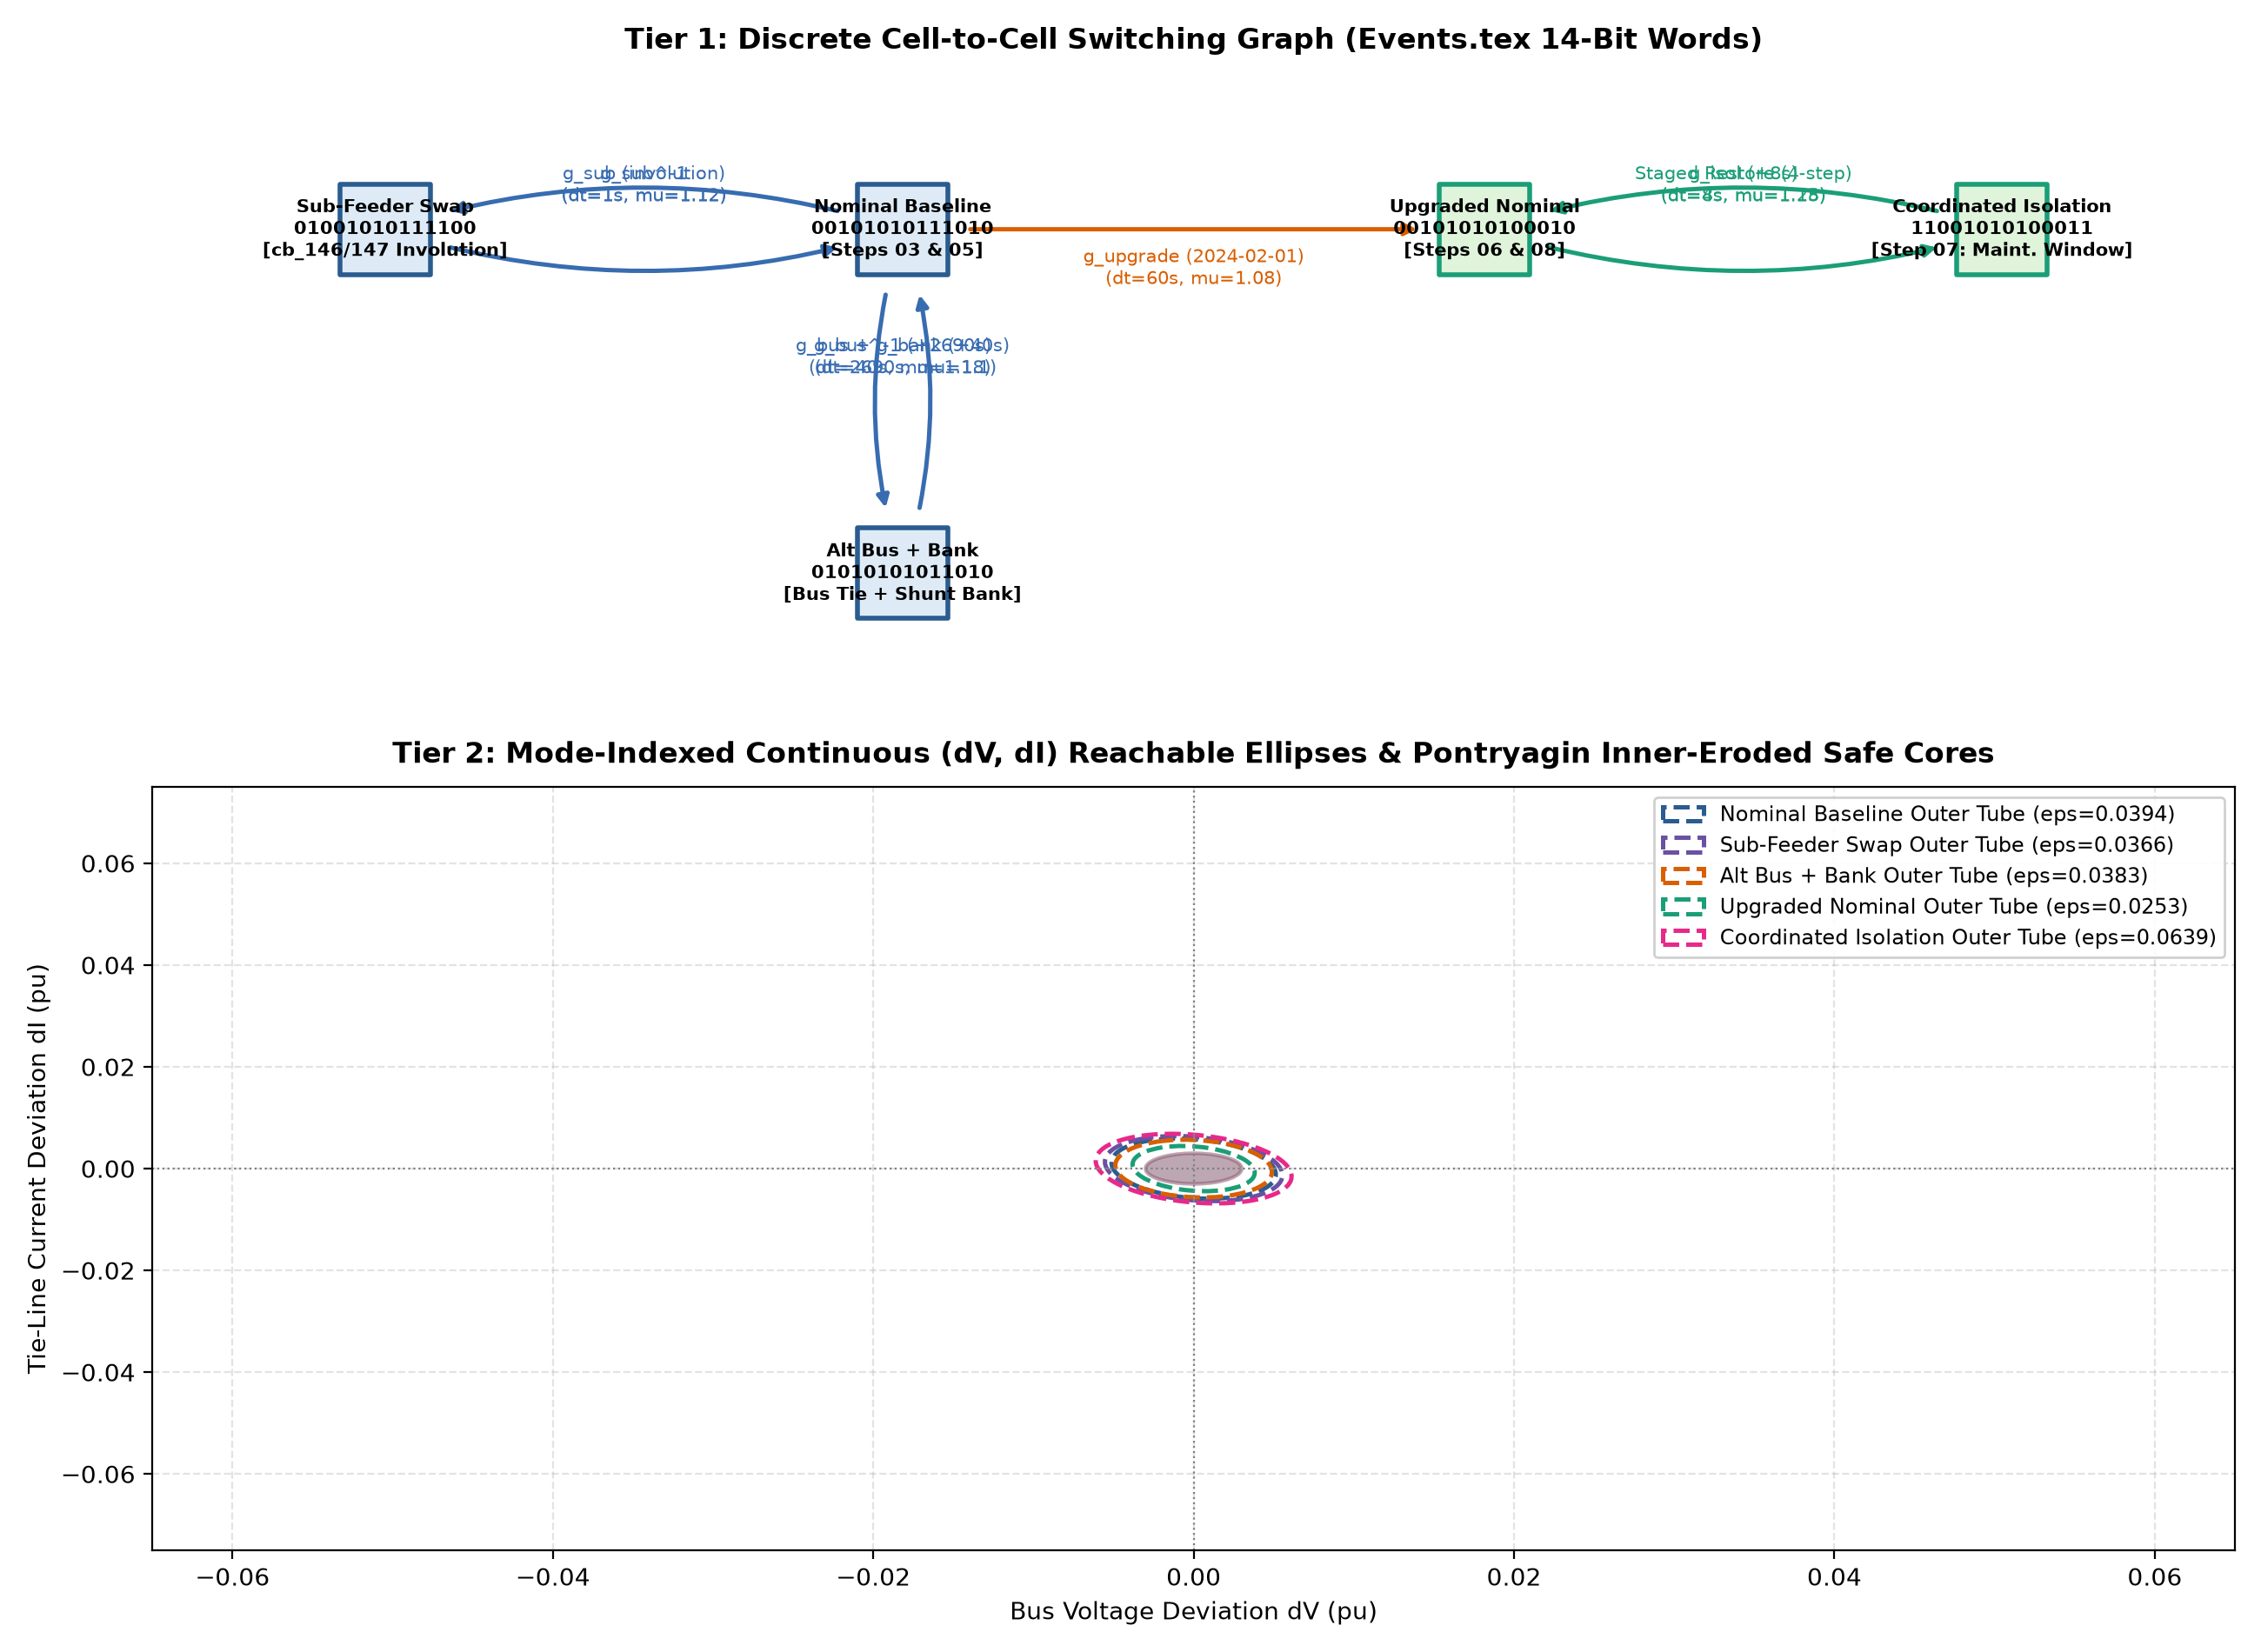
\includegraphics[width=\columnwidth]{hybrid_reachable_set.png}
\caption{Hybrid cotangent reachable set and Pontryagin inner-eroded safe core across Caltech 14-bit switching configurations.}
\label{fig:hybrid_reachable_png}
\end{figure}
\begin{thebibliography}{9}\bibitem{nekrashevych05} V. Nekrashevych, \textit{Self-Similar Groups}, 2005.\bibitem{ramadge87} P. J. Ramadge and W. M. Wonham, \textit{SIAM J. Control Optim.}, 1987.\bibitem{zhong90} H. Zhong and W. M. Wonham, \textit{IEEE TAC}, 1990.\bibitem{hespanha99} J. P. Hespanha and A. S. Morse, \textit{CDC}, 1999.\bibitem{liberzon03} D. Liberzon, \textit{Switching in Systems and Control}, 2003.\bibitem{manchester17} I. R. Manchester and J.-J. E. Slotine, \textit{IEEE TAC}, 2017.\bibitem{shiromoto18} H. S. Shiromoto et al., \textit{IEEE TCNS}, 2019.\bibitem{chen26} J. Y. Chen et al., \textit{ACM e-Energy}, 2026.\end{thebibliography}\n\end{document}